\chapter*{Preface}
\thispagestyle{empty} 


HiFrost is nuclear polarized target apparatus consisting of a dilution refrigerator, internal magnetic coil, microwave guide and NMR coil.  External components of HiFrost include a polarizing magnet, microwave generating EIO, pump and vacuum system to run the dilution refrigerator, and the Q-Meter/Yale Card set up for running the NMR. 


To polarize a target, chemically doped or irradiated beads are placed in the inner-most chamber, the fridge is assembled around the beads and the whole fridge is swung to align with the HIGS gamma beam.  The beads are cooled with liquid helium and polarized with a large external magnet, with an EIO providing microwaves necessary for dynamic nuclear polarization.


To achieve frozen spin mode, the internal magnet is ramped on as the external magnet is ramped off, so eventually the external magnet can be powered down and removed while keeping the polarized beads in a steady magnetic field.

\begin{figure}[h]
 \centering
 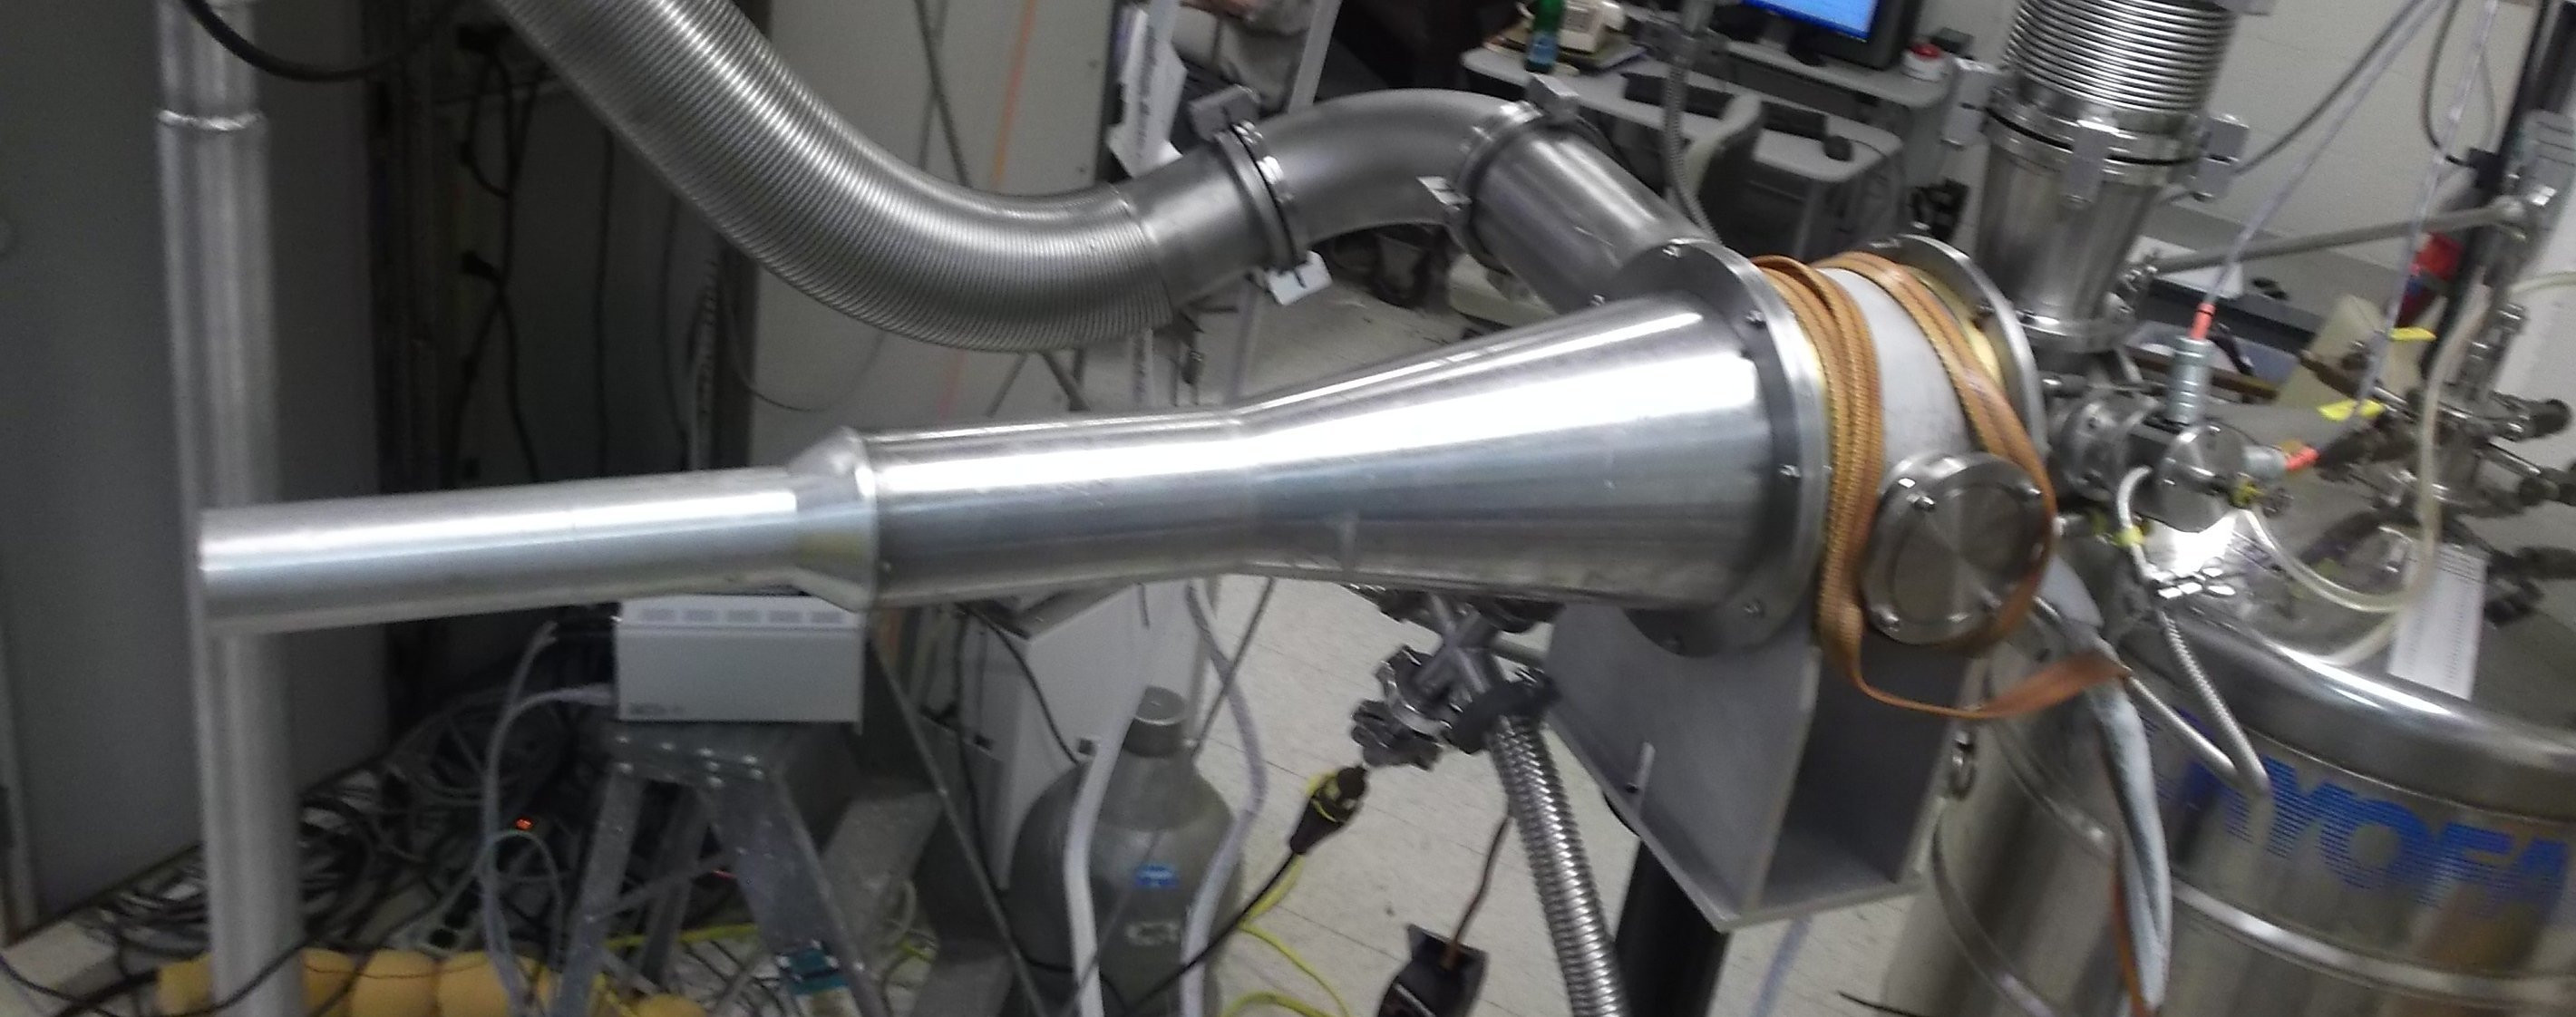
\includegraphics[width=\textwidth]{./img/intro-image.jpg}
 % intro-image.jpg: 0x0 pixel, 0dpi, 0.00x0.00 cm, bb=
 \caption{The HiFrost refrigerator during a test cooldown at UVa.}
 \label{fig:intro-image}
\end{figure}
